% !TeX spellcheck = en_US
% !TeX encoding = UTF-8
\chapter{Code}

\begin{code}
\captionof{listing}{Calculating threshold for pruning}
\label{code:threshold}
\begin{minted}[frame=lines,bgcolor=code_bg,linenos]{python}
weights = []
for param, data in self.named_parameters():
    if 'bias' not in param and key in param:
        weights += list(data.cpu().data.abs().numpy().flatten())
threshold = np.percentile(np.array(weights), percent)
\end{minted}
\end{code}

\begin{code}
\captionof{listing}{Calculating binary mask}
\label{code:mask}
\begin{minted}[frame=lines,bgcolor=code_bg,linenos]{python}
masks = {}
for l, layer in enumerate(self.recurrent_layers):
    masks[l] = []
    for param, data in layer.named_parameters():
        if 'bias' not in param and key in param:
            mask = torch.ones(data.shape,
                              dtype=torch.bool,
                              device=data.device)
            mask[torch.where(abs(data) < threshold)] = False
            masks[l].append(mask)
\end{minted}
\end{code}

% -----------------------------------------------------------------------------------------------------------
% ------------------------------------------------- TABLE ---------------------------------------------------
% -----------------------------------------------------------------------------------------------------------
\chapter{Tables}\label{app:tables}

\begin{table}[h]
	\centering
	\begin{tabular}{|l|c|c|c|c|}
	    \hline
		 & \shortstack{\textbf{All}\\\textbf{ properties}} & \shortstack{\textbf{Only nodes}\\\textbf{ and edges}} & \shortstack{\textbf{Without nodes}\\\textbf{ and edges}} & \shortstack{\textbf{Only}\\\textbf{ variances}}\\
		\hline
		Random Forest $R^{2}$ & 0.61 & 0.71 & -0.05 & 0.06\\
		\hline\hline
		\textbf{Property} & \multicolumn{4}{|l|}{\textbf{Feature importance}}\\
		\hline
		layers & 0.04 & & 0.06 & \\
        nodes & 0.02 & 0.23 & & \\
        edges & 0.01 & 0.29 & & \\
        source\_nodes & 0.08 & 0.29 & & \\
        sink\_nodes & 0.11 & 0.19 & & \\
        diameter & 0.0 & & 0.0 & \\
        density & 0.03 & & 0.03 & \\
        average\_shortest\_path\_length & 0.03 & & 0.03 & \\
        eccentricity\_mean & 0.03 & & 0.04 & \\
        eccentricity\_var & 0.04 & & 0.06 & 0.21 \\
        eccentricity\_std & 0.05 & & 0.09 & \\
        degree\_mean & 0.03 & & 0.03 & \\
        degree\_var & 0.03 & & 0.06 & 0.17 \\
        degree\_std & 0.03 & & 0.04 & \\
        closeness\_mean & 0.04 & & 0.05 & \\
        closeness\_var & 0.07 & & 0.09 & 0.22 \\
        closeness\_std & 0.07 & & 0.08 & \\
        nodes\_betweenness\_mean & 0.05 & & 0.08 & \\
        nodes\_betweenness\_var & 0.08 & & 0.08 & 0.24 \\
        nodes\_betweenness\_std & 0.07 & & 0.07 & \\
        edge\_betweenness\_mean & 0.05 & & 0.06 & \\
        edge\_betweenness\_var & 0.02 & & 0.03 & 0.16 \\
        edge\_betweenness\_std & 0.02 & & 0.02 & \\
		\hline
	\end{tabular}
	\caption[RNN\_ReLU - Feature importance scores for the Random Forest regressor under different circumstances]{Structural properties of the randomly structured RNN\_ReLU's base random graphs and their feature importance scores for the Random Forest regressor under different circumstances.}
	\label{tab:relu_fis}
\end{table}

\begin{table}[h]
	\centering
	\begin{tabular}{|l|c|c|c|c|}
	    \hline
		 & \shortstack{\textbf{All}\\\textbf{ properties}} & \shortstack{\textbf{Only nodes}\\\textbf{ and edges}} & \shortstack{\textbf{Without nodes}\\\textbf{ and edges}} & \shortstack{\textbf{Only}\\\textbf{ variances}}\\
		\hline
		Random Forest $R^{2}$ & 0.87 & 0.75 & 0.78 & 0.76\\
		\hline\hline
		\textbf{Property} & \multicolumn{4}{|l|}{\textbf{Feature importance}}\\
		\hline
		layers & 0.01 & & 0.04 & \\
        nodes & 0.01 & 0.11 & & \\
        edges & 0.01 & 0.12 & & \\
        source\_nodes & 0.67 & 0.71 & & \\
        sink\_nodes & 0.01 & 0.06 & & \\
        diameter & 0.0 & & 0.01 & \\
        density & 0.01 & & 0.02 & \\
        average\_shortest\_path\_length & 0.01 & & 0.02 & \\
        eccentricity\_mean & 0.01 & & 0.02 & \\
        eccentricity\_var & 0.02 & & 0.03 & 0.17 \\
        eccentricity\_std & 0.02 & & 0.03 & \\
        degree\_mean & 0.01 & & 0.03 & \\
        degree\_var & 0.01 & & 0.03 & 0.15 \\
        degree\_std & 0.01 & & 0.03 & \\
        closeness\_mean & 0.01 & & 0.03 & \\
        closeness\_var & 0.02 & & 0.11 & 0.36 \\
        closeness\_std & 0.01 & & 0.16 & \\
        nodes\_betweenness\_mean & 0.04 & & 0.11 & \\
        nodes\_betweenness\_var & 0.01 & & 0.15 & 0.25 \\
        nodes\_betweenness\_std & 0.02 & & 0.14 & \\
        edge\_betweenness\_mean & 0.03 & & 0.03 & \\
        edge\_betweenness\_var & 0.01 & & 0.02 & 0.08 \\
        edge\_betweenness\_std & 0.01 & & 0.02 & \\
		\hline
	\end{tabular}
	\caption[GRU - Feature importance scores for the Random Forest regressor under different circumstances]{Structural properties of the randomly structured GRU's base random graphs and their feature importance scores for the Random Forest regressor under different circumstances.}
	\label{tab:gru_fis}
\end{table}

% -----------------------------------------------------------------------------------------------------------
% ------------------------------------------------- PLOTS ---------------------------------------------------
% -----------------------------------------------------------------------------------------------------------

\chapter{Plots}

\section{Randomly structured RNN\_Tanh}\label{app:rs_tanh}

\begin{figure}[H]
    \centering
    \begin{subfigure}{0.4\textwidth}
        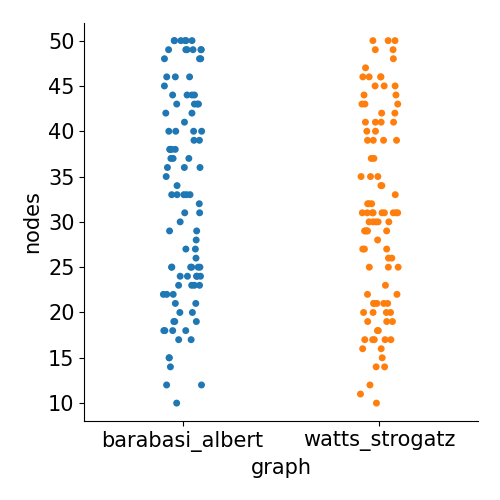
\includegraphics[width=\linewidth]{images/results/random/tanh/graph_nodes.png}
        \caption{} \label{fig:tanh_graph_nodes}
    \end{subfigure}%
    \hfill
    \begin{subfigure}{0.4\textwidth}
        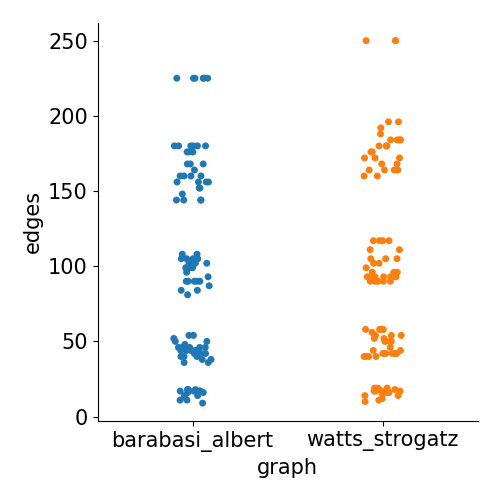
\includegraphics[width=\linewidth]{images/results/random/tanh/graph_edges.png}
        \caption{} \label{fig:tanh_graph_edges}
    \end{subfigure}%
  
    \bigskip
    \begin{subfigure}{0.4\textwidth}
        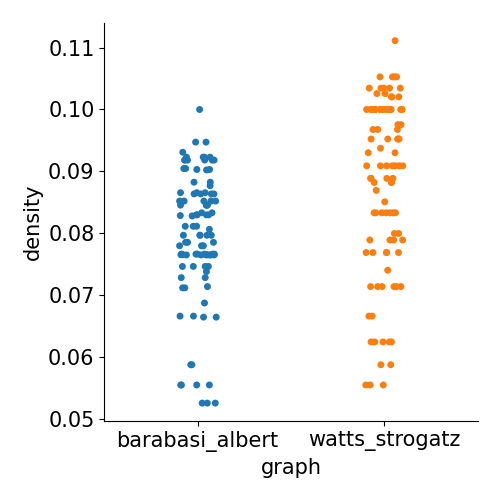
\includegraphics[width=\linewidth]{images/results/random/tanh/graph_density.png}
        \caption{} \label{fig:tanh_graph_density}
    \end{subfigure}
    \hfill
    \begin{subfigure}{0.4\textwidth}
        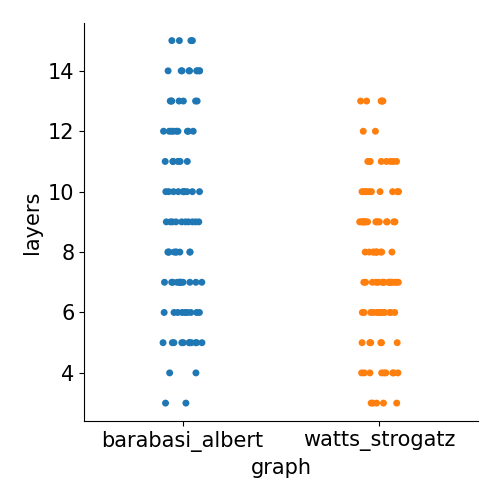
\includegraphics[width=\linewidth]{images/results/random/tanh/graph_layers.png}
        \caption{} \label{fig:tanh_graph_layers}
    \end{subfigure}

\caption[Comparison of basic graph properties and number of layers in WS and BA based RNN\_Tanh models]{Comparison of basic graph properties and number of layers in Watts–Strogatz and Barabási–Albert based RNN\_Tanh models} \label{fig:tanh_graphs}
\end{figure}

\begin{figure}[H]
    \centering
    \begin{subfigure}{0.45\textwidth}
        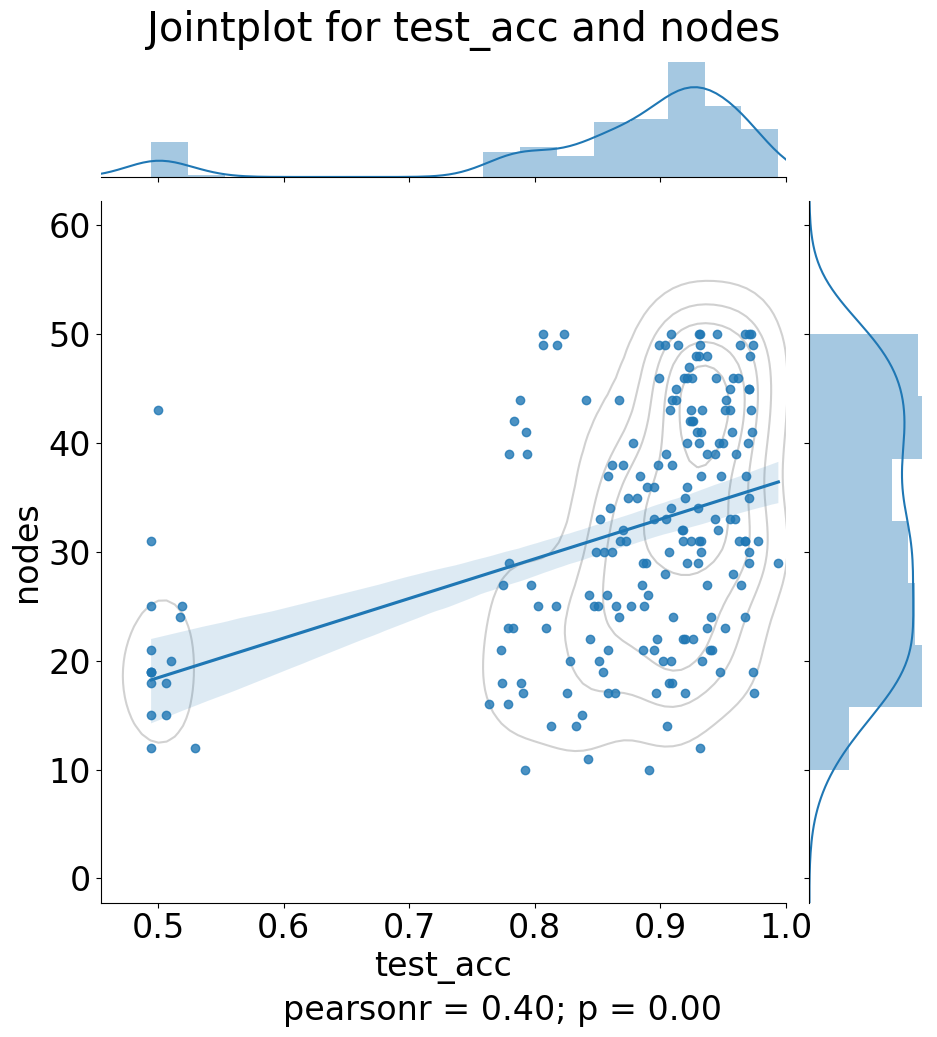
\includegraphics[width=\linewidth]{images/results/random/tanh/jointplot_test_acc_nodes.png}
        \caption{Correlation between test\_acc and the number of nodes} \label{fig:jp_tanh_node}
    \end{subfigure}%
    \hfill
    \begin{subfigure}{0.45\textwidth}
        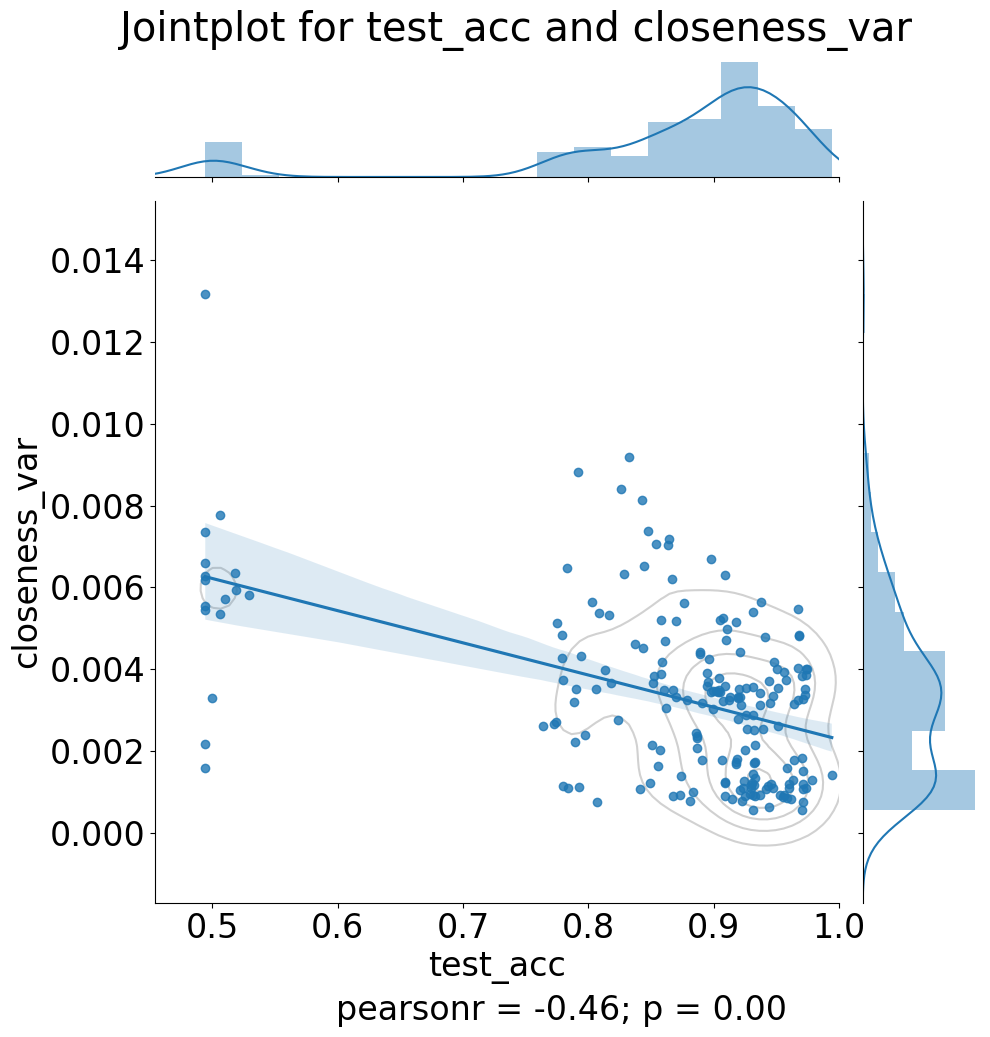
\includegraphics[width=\linewidth]{images/results/random/tanh/jointplot_test_acc_closeness_var.png}
        \caption{Correlation between test\_acc and closeness in base random graph} \label{fig:jp_tanh_close}
    \end{subfigure}%
  
    \bigskip
    \begin{subfigure}{0.45\textwidth}
        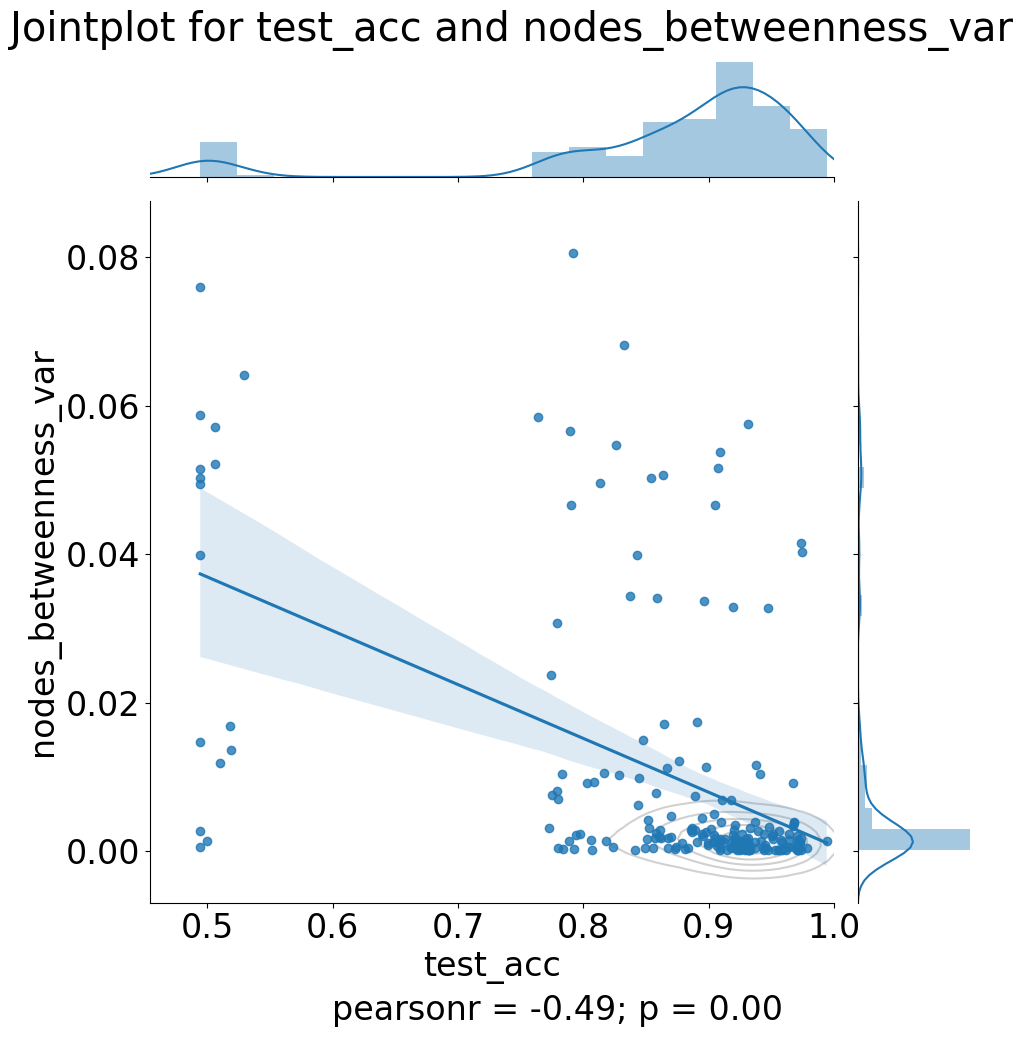
\includegraphics[width=\linewidth]{images/results/random/tanh/jointplot_test_acc_nodes_betweenness_var.png}
        \caption{Correlation between test\_acc and node betweenness in base random graph} \label{fig:jp_tanh_between}
    \end{subfigure}
    \hfill
    \begin{subfigure}{0.45\textwidth}
        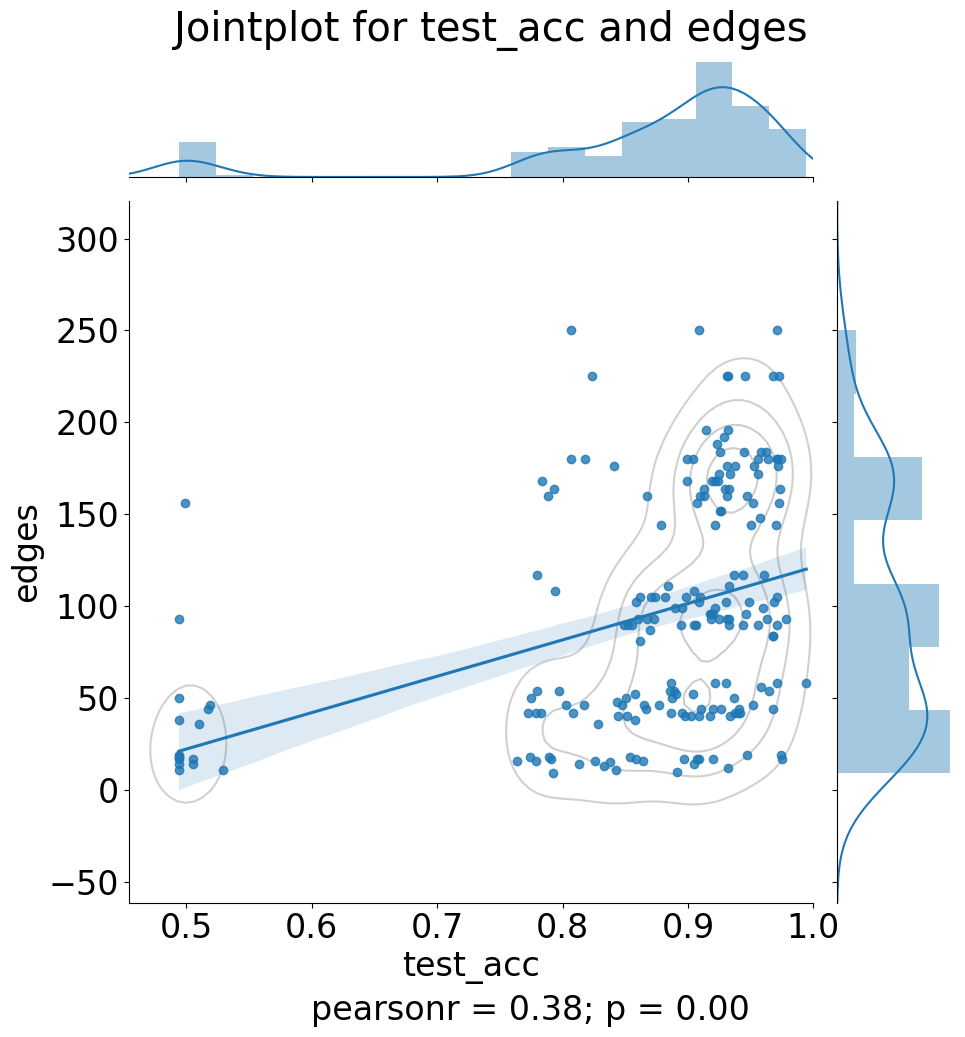
\includegraphics[width=\linewidth]{images/results/random/tanh/jointplot_test_acc_edges.png}
        \caption{Correlation between test\_acc and the number of edges} \label{fig:jp_tanh_edge}
    \end{subfigure}%
    

\caption[Correlation between test accuracy of RNN\_Tanh and its different graph and recurrent network properties - 1]{Correlation between test accuracy of RNN\_Tanh and its different graph and recurrent network properties} \label{fig:tanh_correlation}
\end{figure}

\newpage
\section{Randomly structured RNN\_ReLU}\label{app:rs_relu}

\begin{figure}[H]
    \centering
    \begin{subfigure}{0.45\textwidth}
        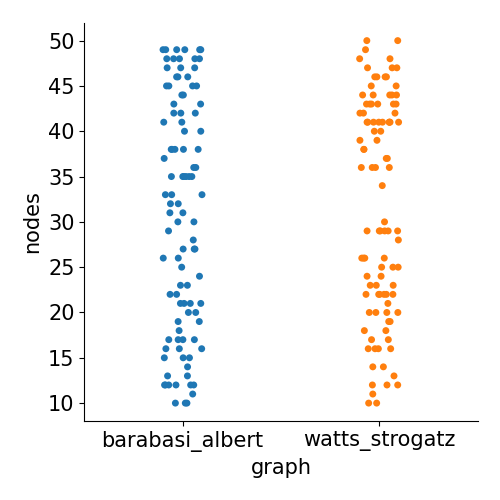
\includegraphics[width=\linewidth]{images/results/random/relu/graph_nodes.png}
        \caption{} \label{fig:relu_graph_nodes}
    \end{subfigure}%
    \hfill
    \begin{subfigure}{0.45\textwidth}
        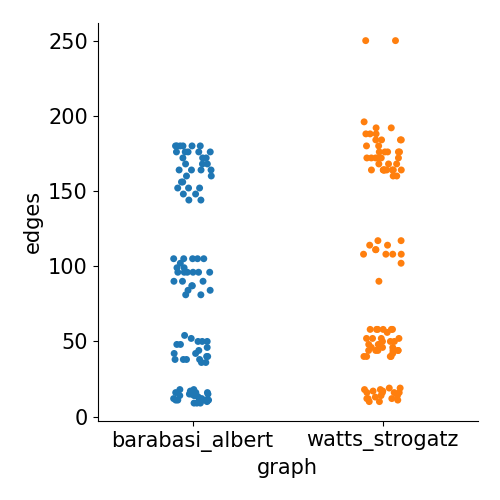
\includegraphics[width=\linewidth]{images/results/random/relu/graph_edges.png}
        \caption{} \label{fig:relu_graph_edges}
    \end{subfigure}%
  
    \bigskip
    \begin{subfigure}{0.45\textwidth}
        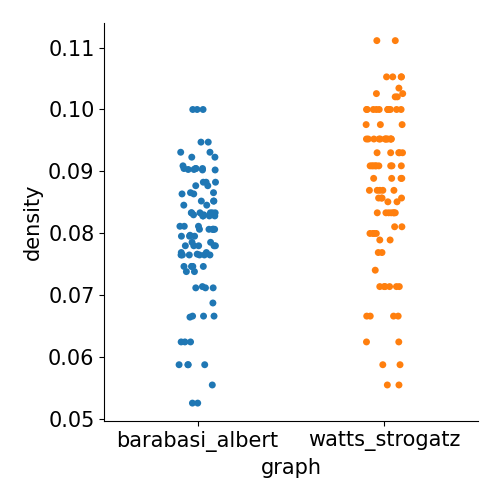
\includegraphics[width=\linewidth]{images/results/random/relu/graph_density.png}
        \caption{} \label{fig:relu_graph_density}
    \end{subfigure}
    \hfill
    \begin{subfigure}{0.45\textwidth}
        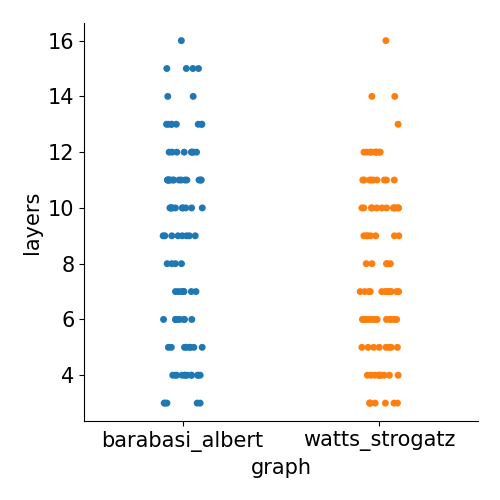
\includegraphics[width=\linewidth]{images/results/random/relu/graph_layers.png}
        \caption{} \label{fig:relu_graph_layers}
    \end{subfigure}

\caption[Comparison of basic graph properties and number of layers in WS and BA based RNN\_ReLU models]{Comparison of basic graph properties and number of layers in Watts–Strogatz and Barabási–Albert based RNN\_ReLU models} \label{fig:relu_graphs}
\end{figure}

\begin{figure}[H]
    \centering
    \begin{subfigure}{0.45\textwidth}
        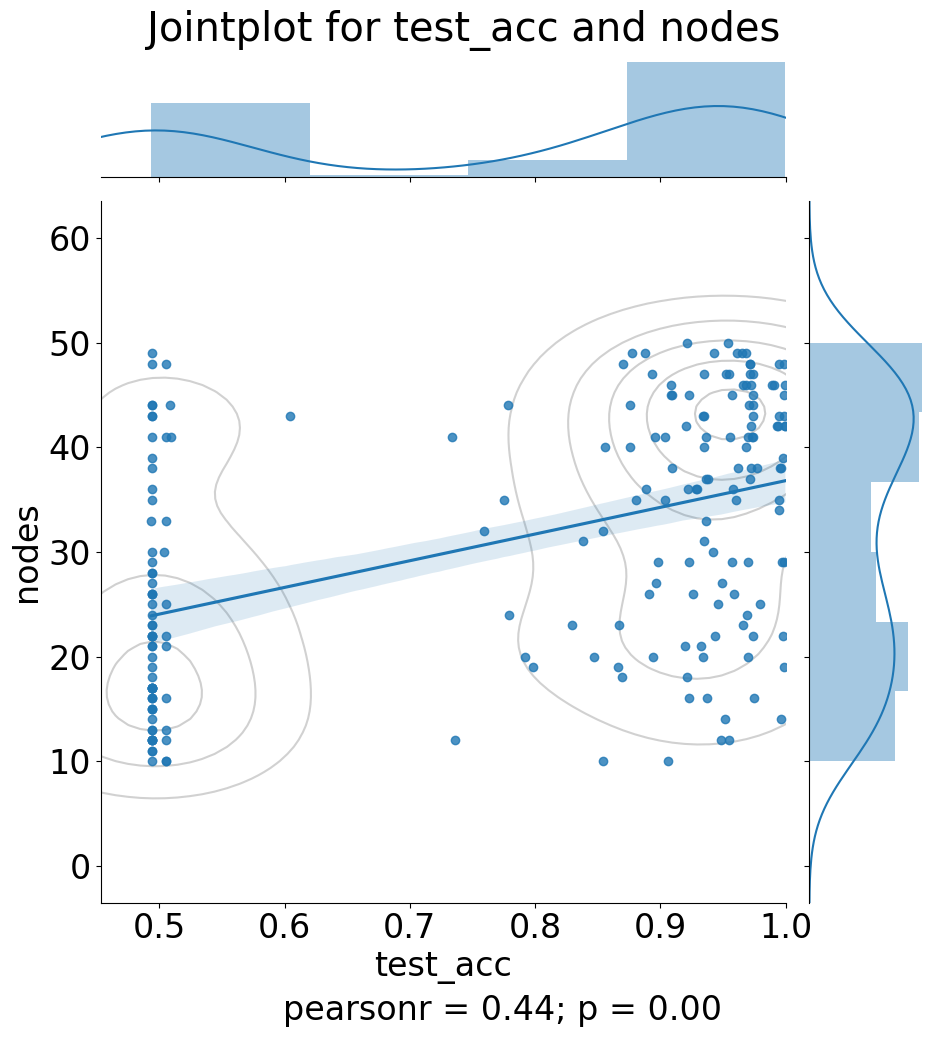
\includegraphics[width=\linewidth]{images/results/random/relu/jointplot_test_acc_nodes.png}
        \caption{Correlation between test\_acc and the number of nodes} \label{fig:jp_relu_node}
    \end{subfigure}%
    \hfill
    \begin{subfigure}{0.45\textwidth}
        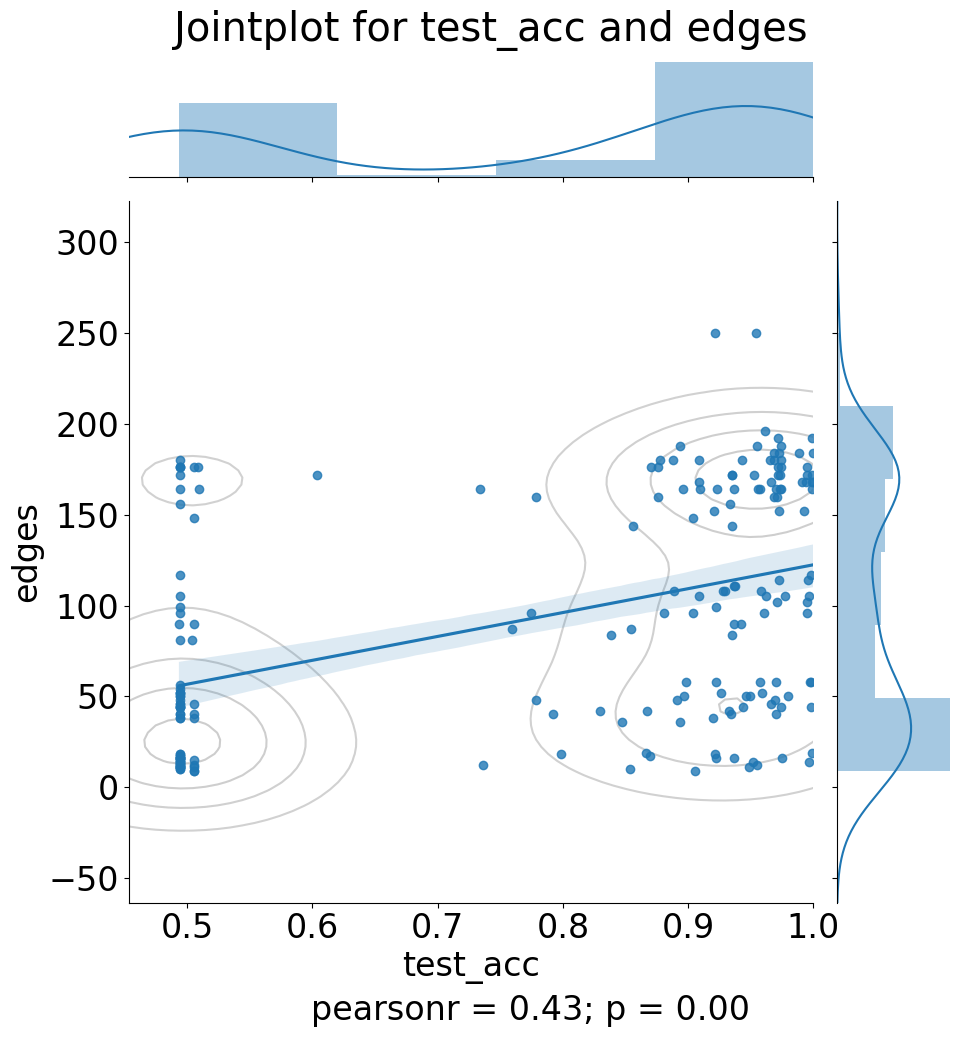
\includegraphics[width=\linewidth]{images/results/random/relu/jointplot_test_acc_edges.png}
        \caption{Correlation between test\_acc and the number of edges} \label{fig:jp_relu_edge}
    \end{subfigure}%
  
    \bigskip
    \begin{subfigure}{0.45\textwidth}
        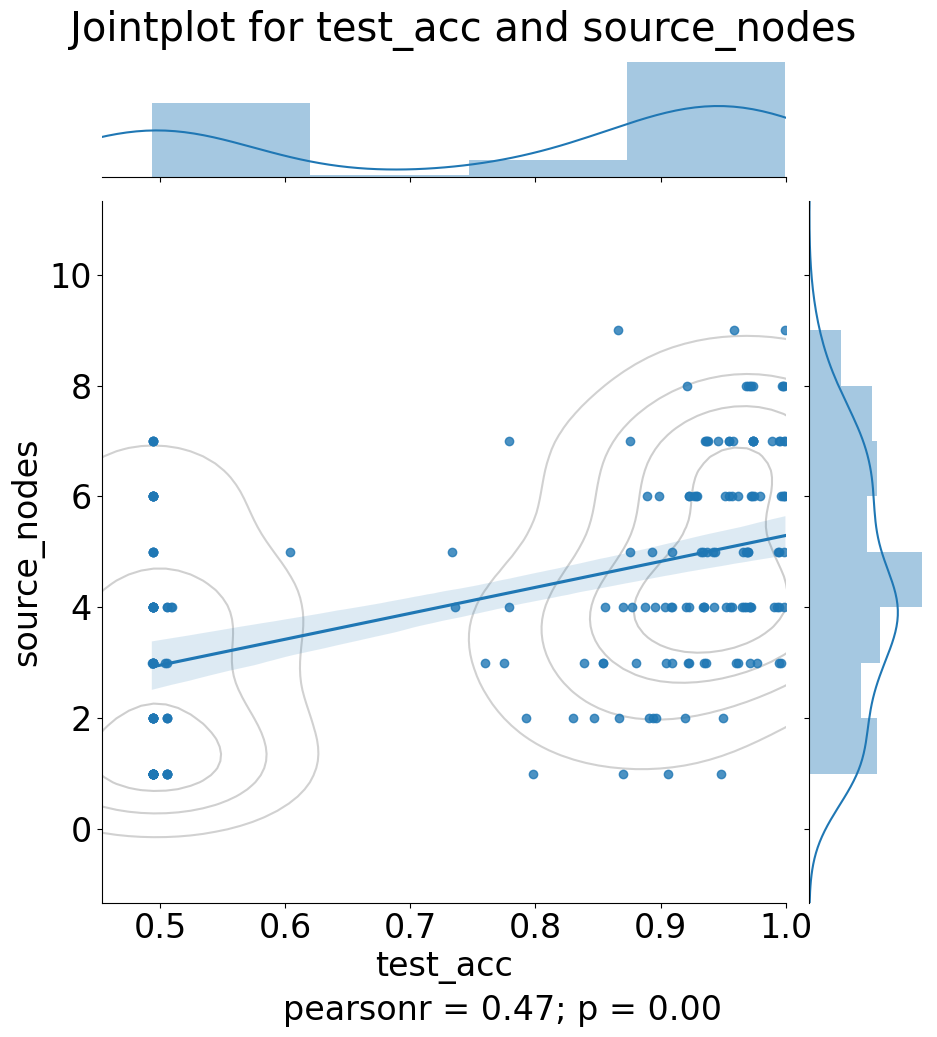
\includegraphics[width=\linewidth]{images/results/random/relu/jointplot_test_acc_source_nodes.png}
        \caption{Correlation between test\_acc and the number of source nodes} \label{fig:jp_relu_source}
    \end{subfigure}
    \hfill
    \begin{subfigure}{0.45\textwidth}
        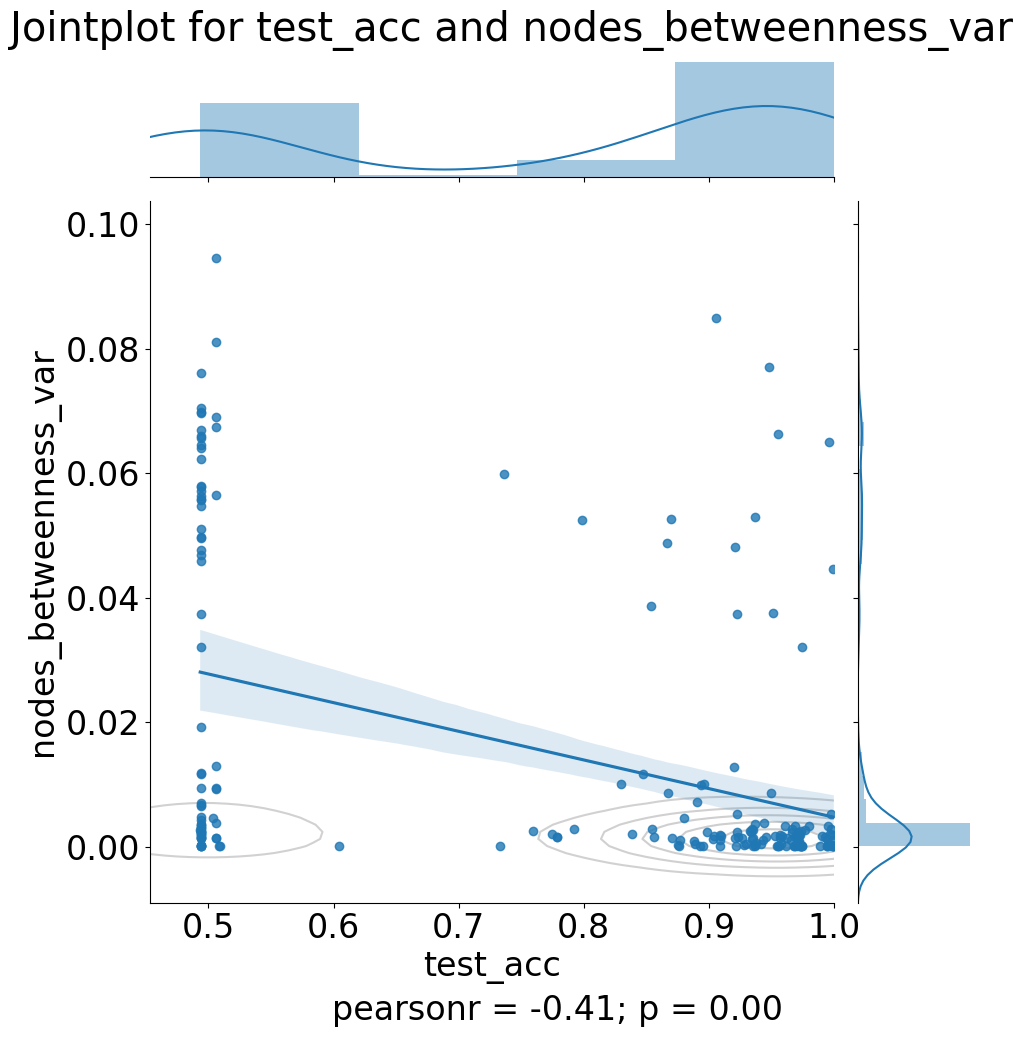
\includegraphics[width=\linewidth]{images/results/random/relu/jointplot_test_acc_nodes_betweenness_var.png}
        \caption{Correlation between test\_acc and node betweenness in base random graph} \label{fig:jp_relu_between}
    \end{subfigure}

\caption[Correlation between test accuracy of RNN\_ReLU and its different graph and recurrent network properties - 1]{Correlation between test accuracy of RNN\_ReLU and its different graph and recurrent network properties} \label{fig:relu_correlation}
\end{figure}

\newpage
\section{Randomly structured LSTM}\label{app:rs_lstm}

\begin{figure}[H]
    \centering
    \begin{subfigure}{0.45\textwidth}
        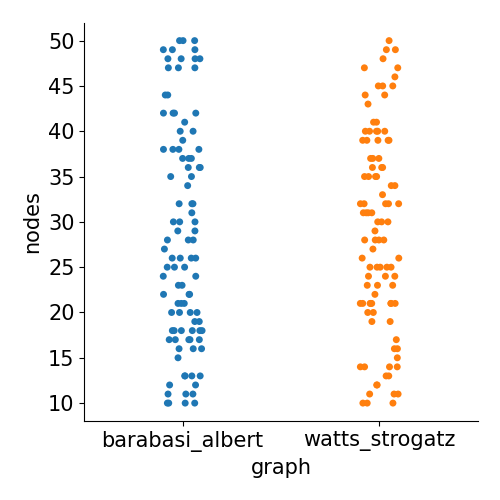
\includegraphics[width=\linewidth]{images/results/random/lstm/graph_nodes.png}
        \caption{} \label{fig:lstm_graph_nodes}
    \end{subfigure}%
    \hfill
    \begin{subfigure}{0.45\textwidth}
        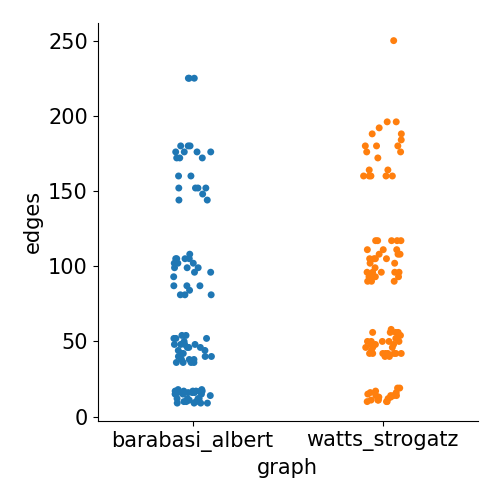
\includegraphics[width=\linewidth]{images/results/random/lstm/graph_edges.png}
        \caption{} \label{fig:lstm_graph_edges}
    \end{subfigure}%
  
    \bigskip
    \begin{subfigure}{0.45\textwidth}
        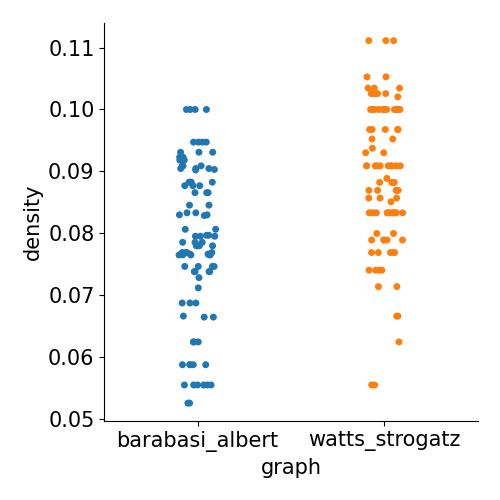
\includegraphics[width=\linewidth]{images/results/random/lstm/graph_density.png}
        \caption{} \label{fig:lstm_graph_density}
    \end{subfigure}
    \hfill
    \begin{subfigure}{0.45\textwidth}
        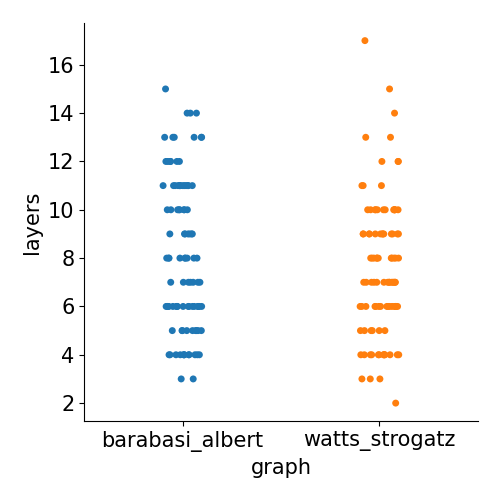
\includegraphics[width=\linewidth]{images/results/random/lstm/graph_layers.png}
        \caption{} \label{fig:lstm_graph_layers}
    \end{subfigure}

\caption[Comparison of basic graph properties and number of layers in WS and BA based LSTM models]{Comparison of basic graph properties and number of layers in Watts–Strogatz and Barabási–Albert based LSTM models} \label{fig:lstm_graphs}
\end{figure}

\begin{figure}[H]
    \centering
    \begin{subfigure}{0.45\textwidth}
        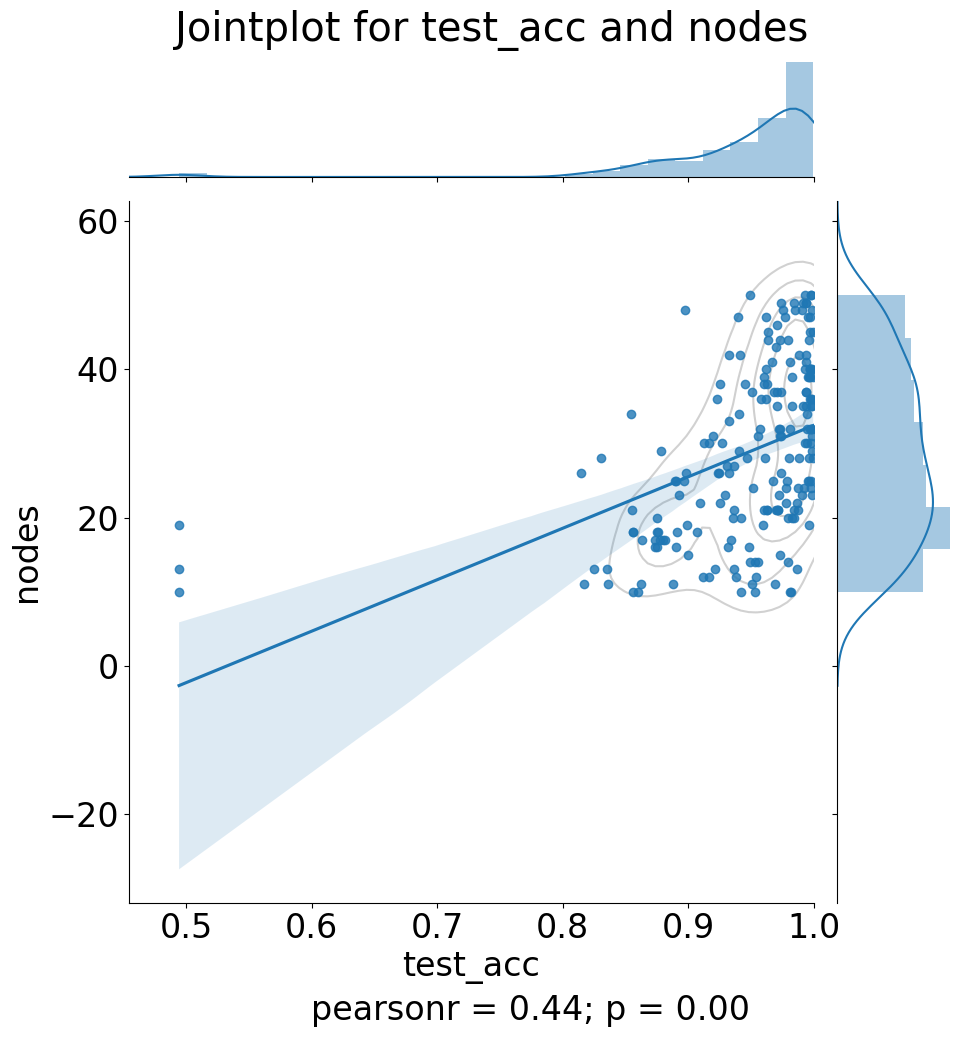
\includegraphics[width=\linewidth]{images/results/random/lstm/jointplot_test_acc_nodes.png}
        \caption{Correlation between test\_acc and the number of nodes} \label{fig:jp_lstm_node}
    \end{subfigure}%
    \hfill
    \begin{subfigure}{0.45\textwidth}
        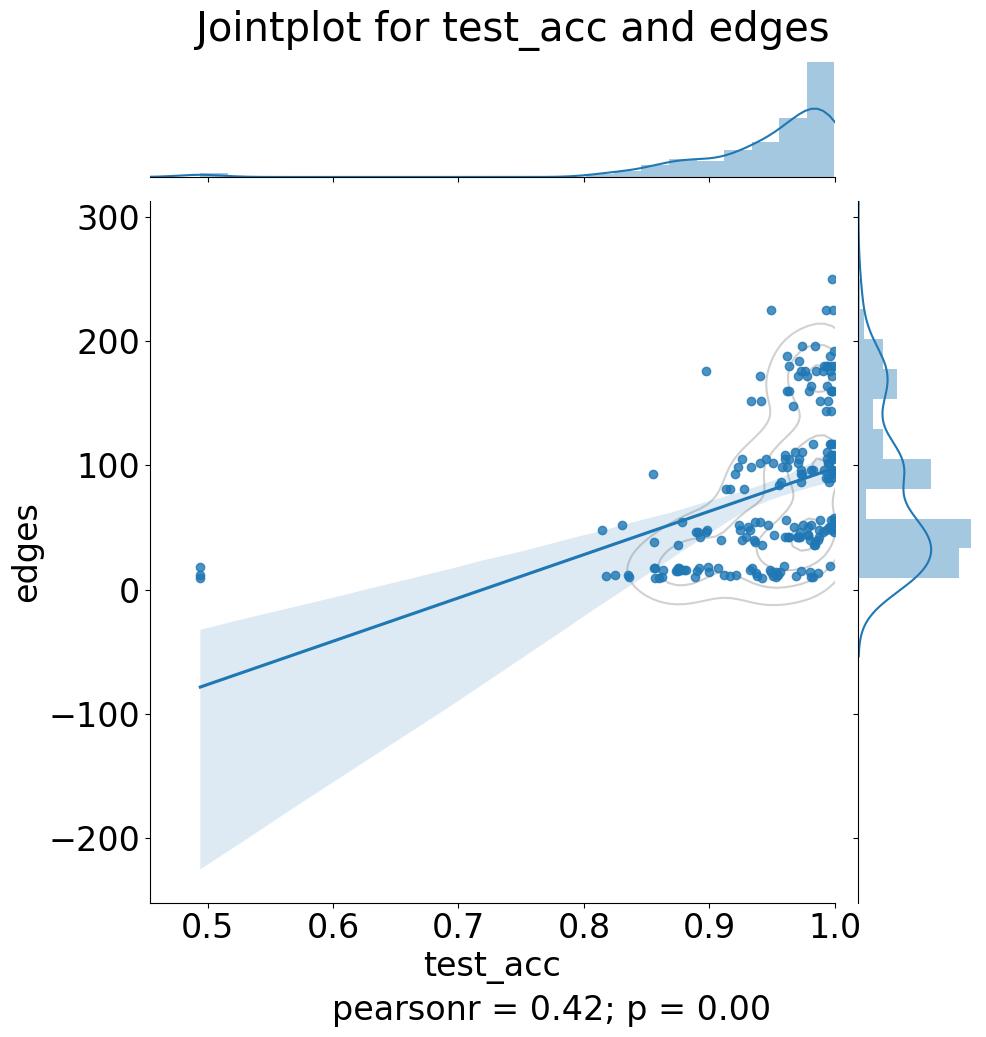
\includegraphics[width=\linewidth]{images/results/random/lstm/jointplot_test_acc_edges.png}
        \caption{Correlation between test\_acc and the number of edges} \label{fig:jp_lstm_edge}
    \end{subfigure}%
  
    \bigskip
    \begin{subfigure}{0.45\textwidth}
        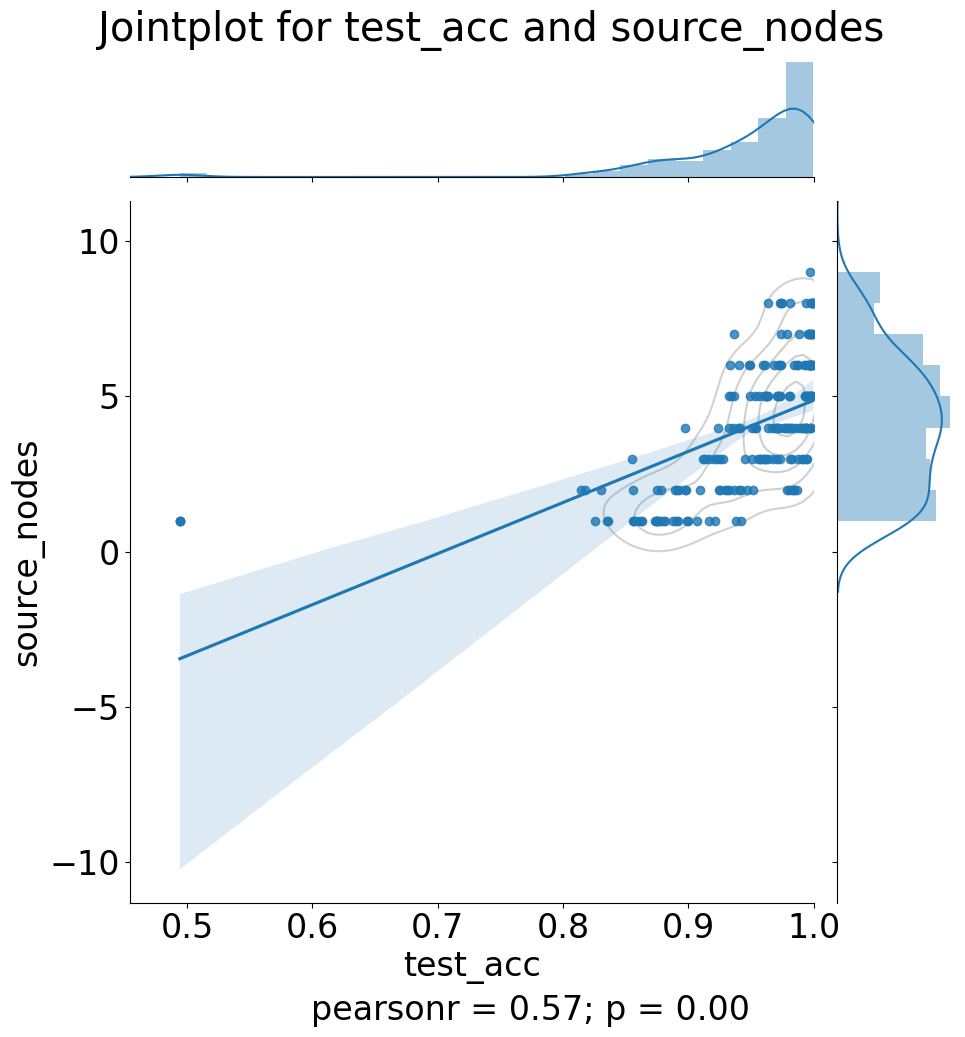
\includegraphics[width=\linewidth]{images/results/random/lstm/jointplot_test_acc_source_nodes.png}
        \caption{Correlation between test\_acc and the number of source nodes} \label{fig:jp_lstm_source}
    \end{subfigure}
    \hfill
    \begin{subfigure}{0.45\textwidth}
        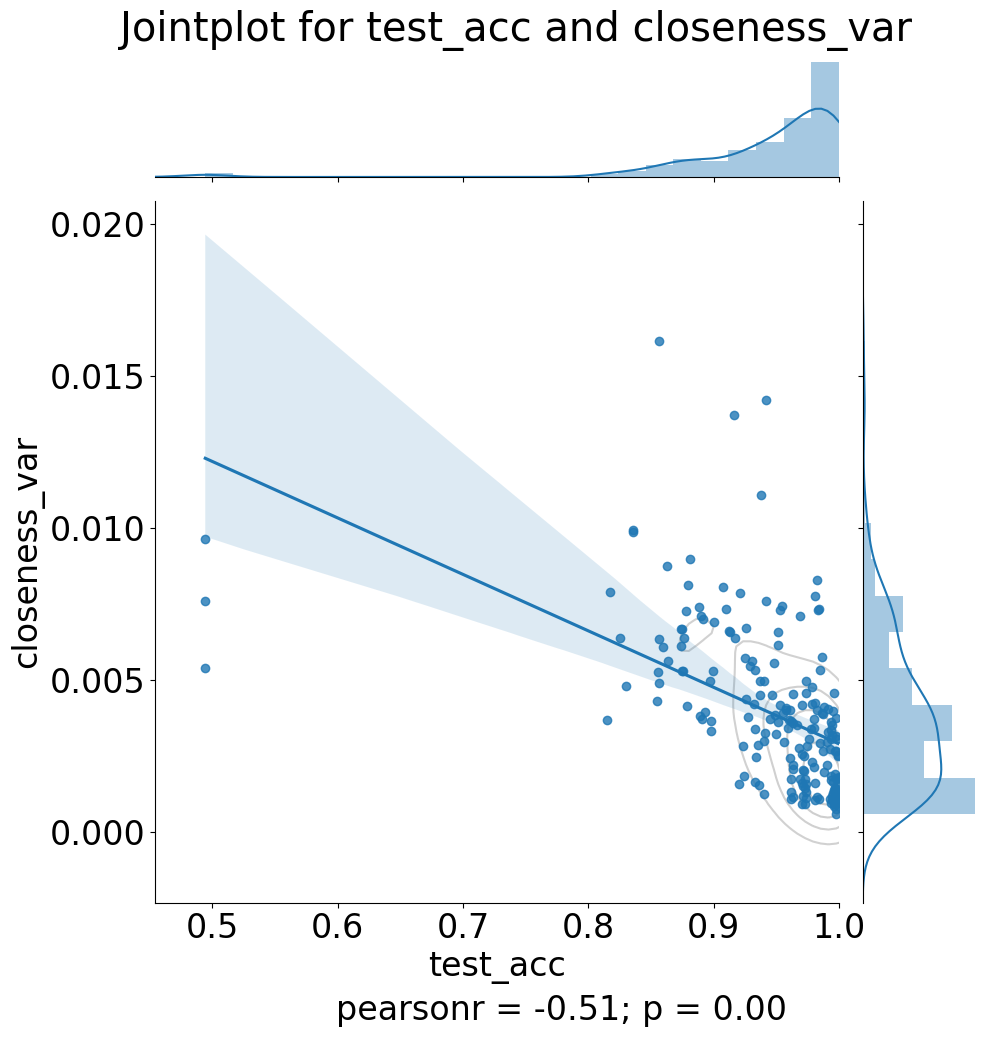
\includegraphics[width=\linewidth]{images/results/random/lstm/jointplot_test_acc_closeness_var.png}
        \caption{Correlation between test\_acc and closeness in base random graph} \label{fig:jp_lstm_close}
    \end{subfigure}

\caption[Correlation between test accuracy of LSTM and its different graph and recurrent network properties - 1]{Correlation between test accuracy of LSTM and its different graph and recurrent network properties - 1} \label{fig:lstm_correlation_1}
\end{figure}

\begin{figure}[H]
    \centering
    \begin{subfigure}{0.45\textwidth}
        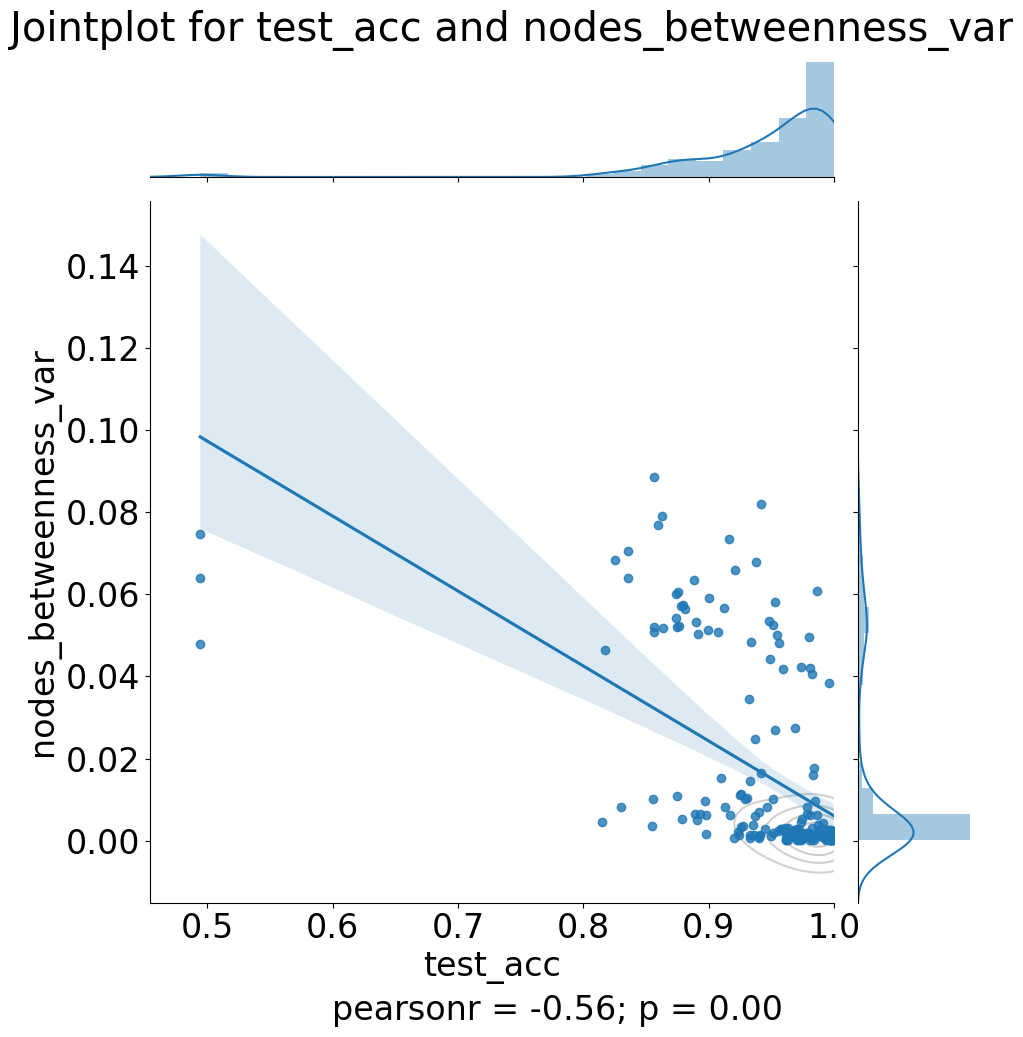
\includegraphics[width=\linewidth]{images/results/random/lstm/jointplot_test_acc_nodes_betweenness_var.png}
        \caption{Correlation between test\_acc and node betweenness in base random graph} \label{fig:jp_lstm_node_bn}
    \end{subfigure}
    \hfill
    \begin{subfigure}{0.45\textwidth}
        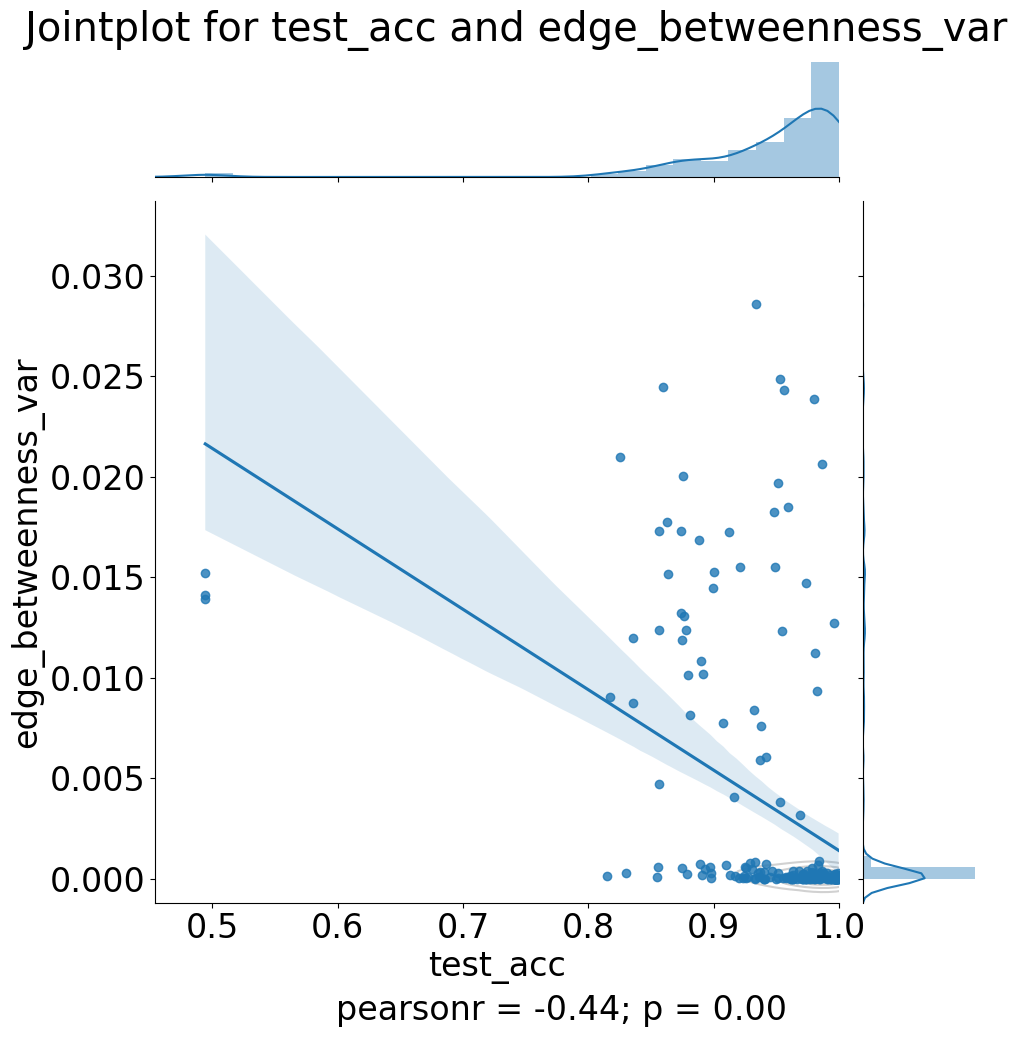
\includegraphics[width=\linewidth]{images/results/random/lstm/jointplot_test_acc_edge_betweenness_var.png}
        \caption{Correlation between test\_acc and edge betweenness in base random graph} \label{fig:jp_lstm_edge_bn}
    \end{subfigure}

\caption[Correlation between test accuracy of LSTM and its different graph and recurrent network properties - 2]{Correlation between test accuracy of LSTM and its different graph and recurrent network properties - 2} \label{fig:lstm_correlation_2}
\end{figure}

\newpage
\section{Randomly structured GRU}\label{app:rs_gru}

\begin{figure}[H]
    \centering
    \begin{subfigure}{0.45\textwidth}
        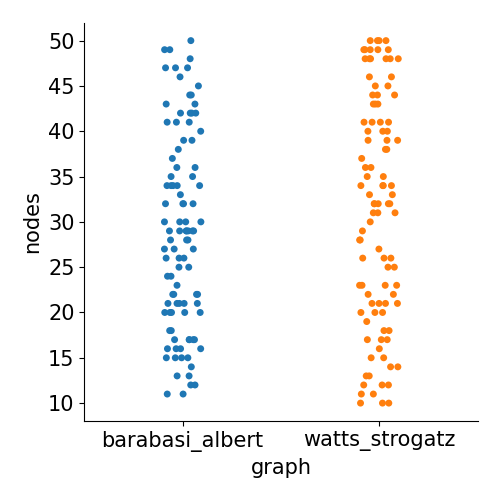
\includegraphics[width=\linewidth]{images/results/random/gru/graph_nodes.png}
        \caption{} \label{fig:gru_graph_nodes}
    \end{subfigure}%
    \hfill
    \begin{subfigure}{0.45\textwidth}
        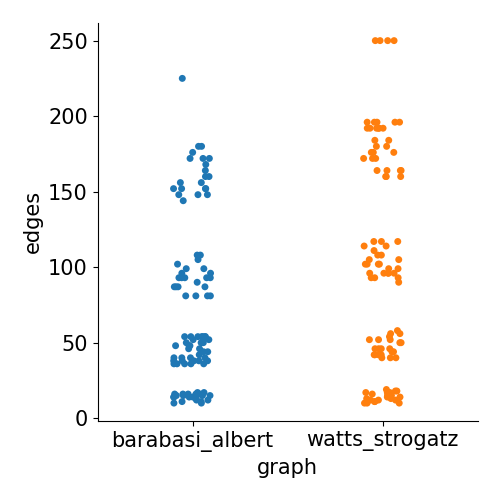
\includegraphics[width=\linewidth]{images/results/random/gru/graph_edges.png}
        \caption{} \label{fig:gru_graph_edges}
    \end{subfigure}%
  
    \bigskip
    \begin{subfigure}{0.45\textwidth}
        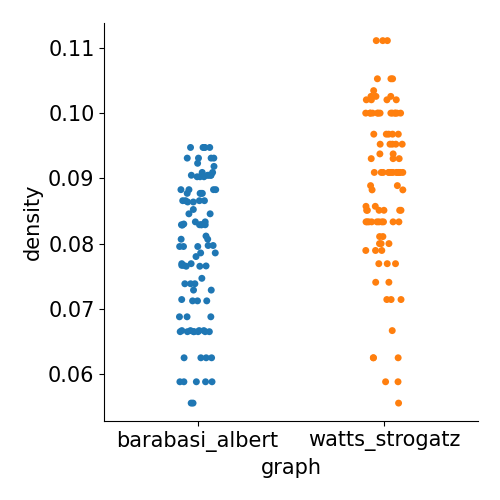
\includegraphics[width=\linewidth]{images/results/random/gru/graph_density.png}
        \caption{} \label{fig:gru_graph_density}
    \end{subfigure}
    \hfill
    \begin{subfigure}{0.45\textwidth}
        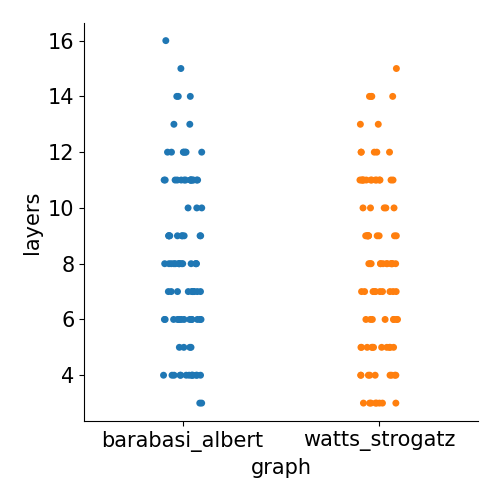
\includegraphics[width=\linewidth]{images/results/random/gru/graph_layers.png}
        \caption{} \label{fig:gru_graph_layers}
    \end{subfigure}

\caption[Comparison of basic graph properties and number of layers in WS and BA based GRU models]{Comparison of basic graph properties and number of layers in Watts–Strogatz and Barabási–Albert based GRU models} \label{fig:gru_graphs}
\end{figure}

\begin{figure}[H]
    \centering
    \begin{subfigure}{0.45\textwidth}
        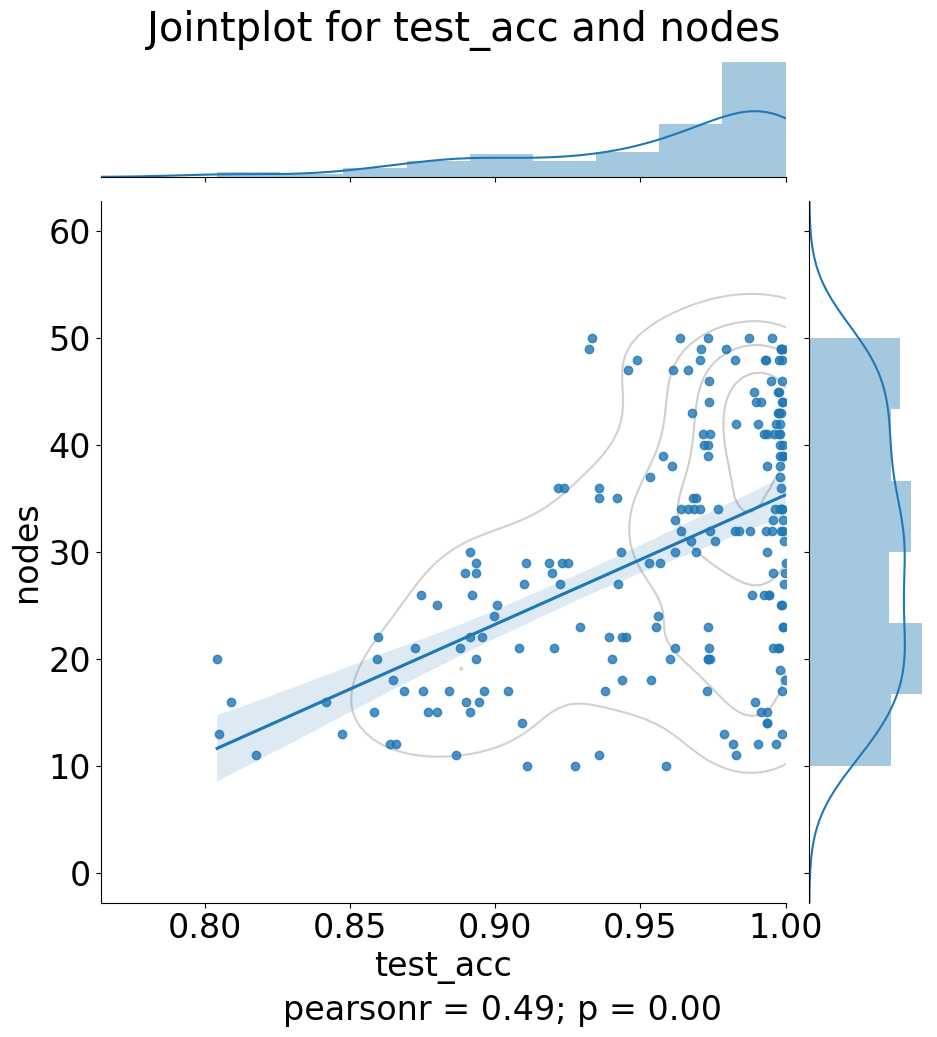
\includegraphics[width=\linewidth]{images/results/random/gru/jointplot_test_acc_nodes.png}
        \caption{Correlation between test\_acc and the number of nodes} \label{fig:jp_gru_node}
    \end{subfigure}%
    \hfill
    \begin{subfigure}{0.45\textwidth}
        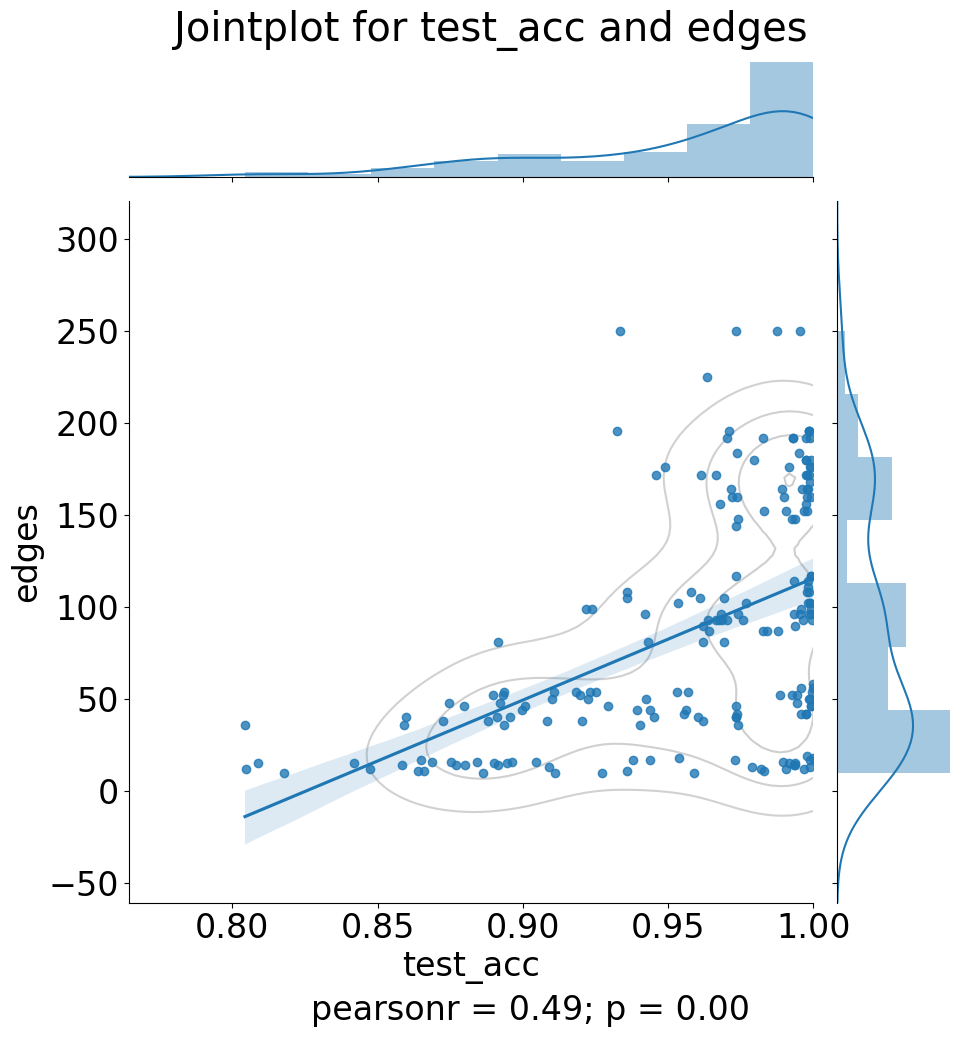
\includegraphics[width=\linewidth]{images/results/random/gru/jointplot_test_acc_edges.png}
        \caption{Correlation between test\_acc and the number of edges} \label{fig:jp_gru_edge}
    \end{subfigure}%
  
    \bigskip
    \begin{subfigure}{0.45\textwidth}
        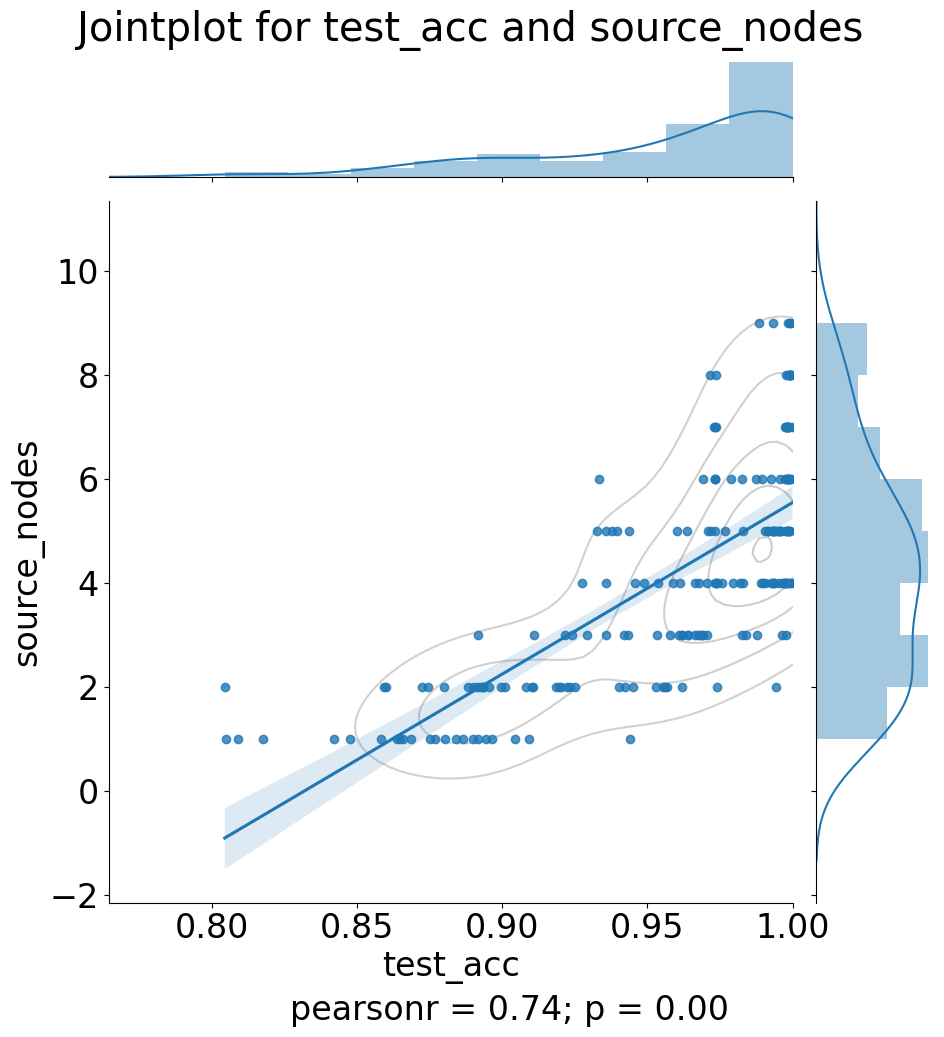
\includegraphics[width=\linewidth]{images/results/random/gru/jointplot_test_acc_source_nodes.png}
        \caption{Correlation between test\_acc and the number of source nodes} \label{fig:jp_gru_source}
    \end{subfigure}
    \hfill
    \begin{subfigure}{0.45\textwidth}
        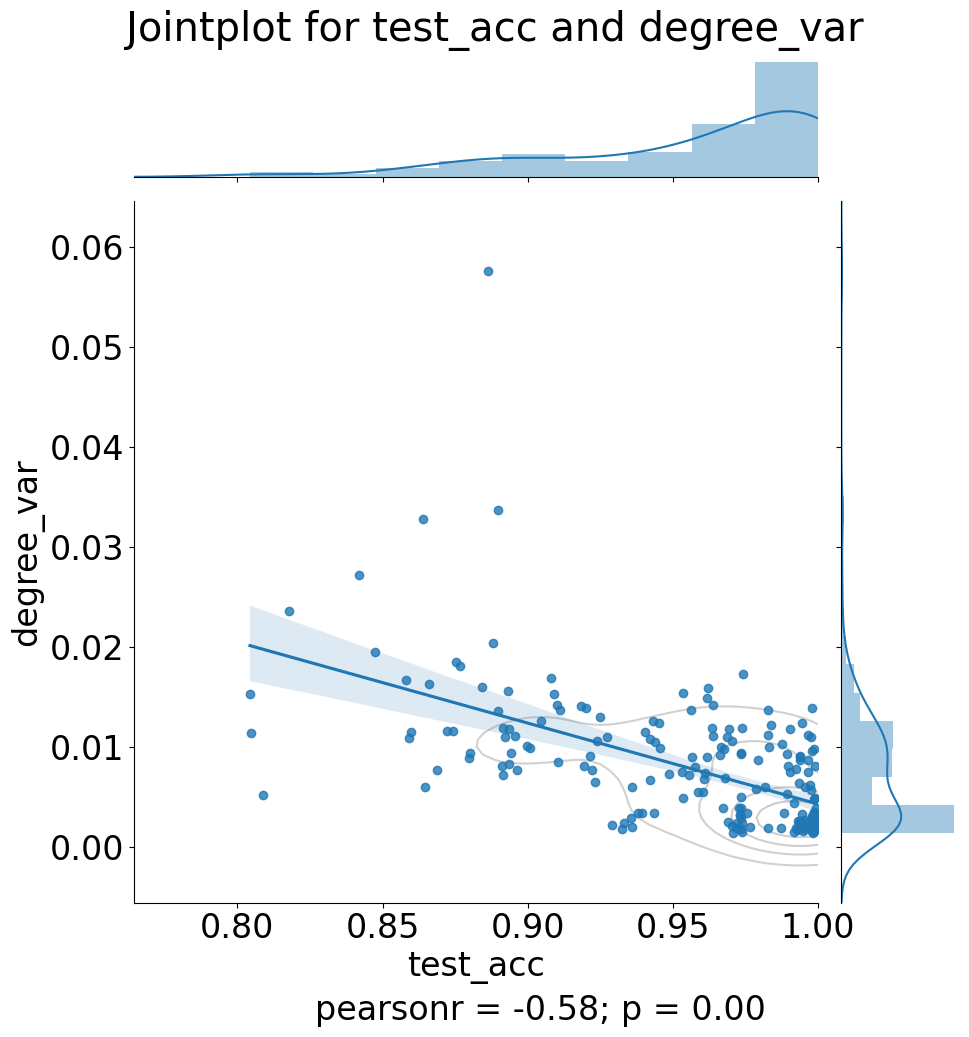
\includegraphics[width=\linewidth]{images/results/random/gru/jointplot_test_acc_degree_var.png}
        \caption{Correlation between test\_acc and degree of the base random graph} \label{fig:jp_gru_degree}
    \end{subfigure}

\caption[Correlation between test accuracy of GRU and its different graph and recurrent network properties - 1]{Correlation between test accuracy of GRU and its different graph and recurrent network properties - 1} \label{fig:gru_correlation_1}
\end{figure}

\begin{figure}[H]
    \centering
    \begin{subfigure}{0.45\textwidth}
        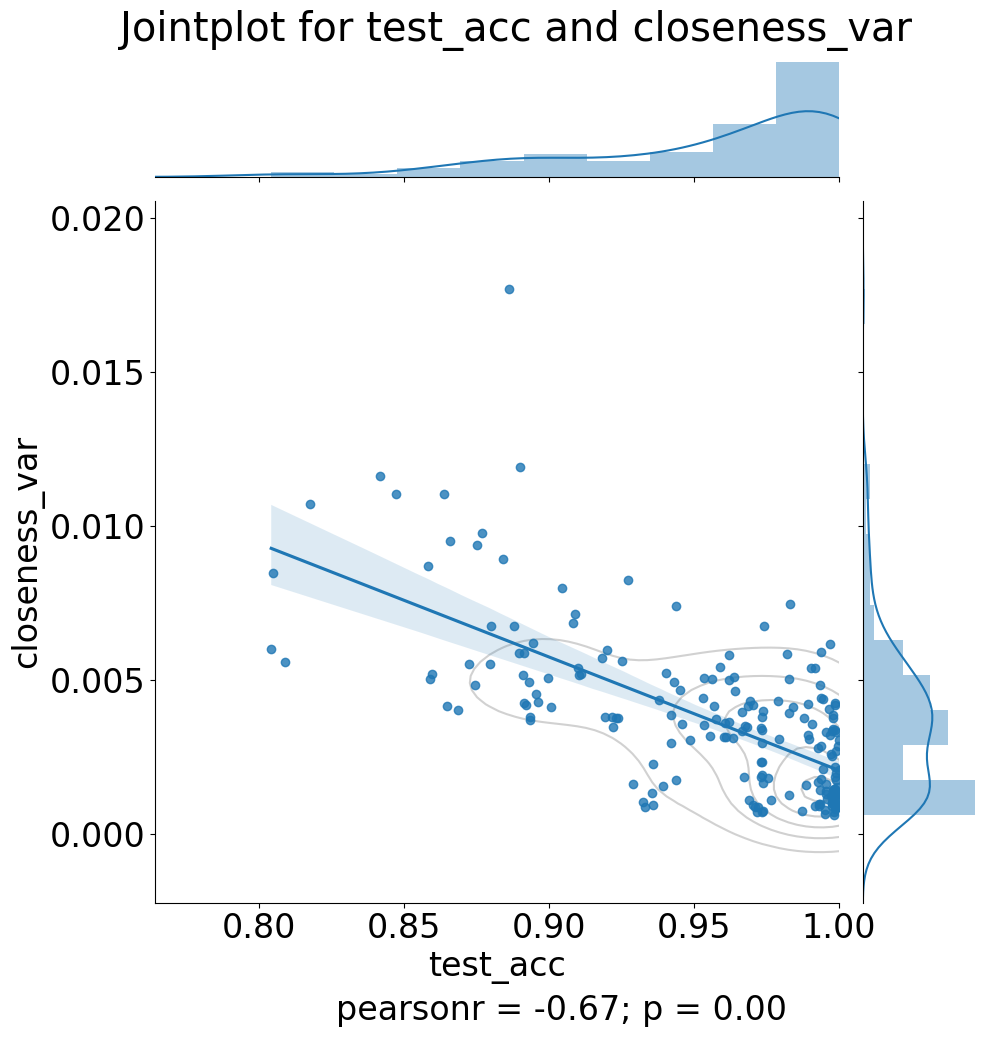
\includegraphics[width=\linewidth]{images/results/random/gru/jointplot_test_acc_closeness_var.png}
        \caption{Correlation between test\_acc and closeness in base random graph} \label{fig:jp_gru_close}
    \end{subfigure}
    \hfill
    \begin{subfigure}{0.45\textwidth}
        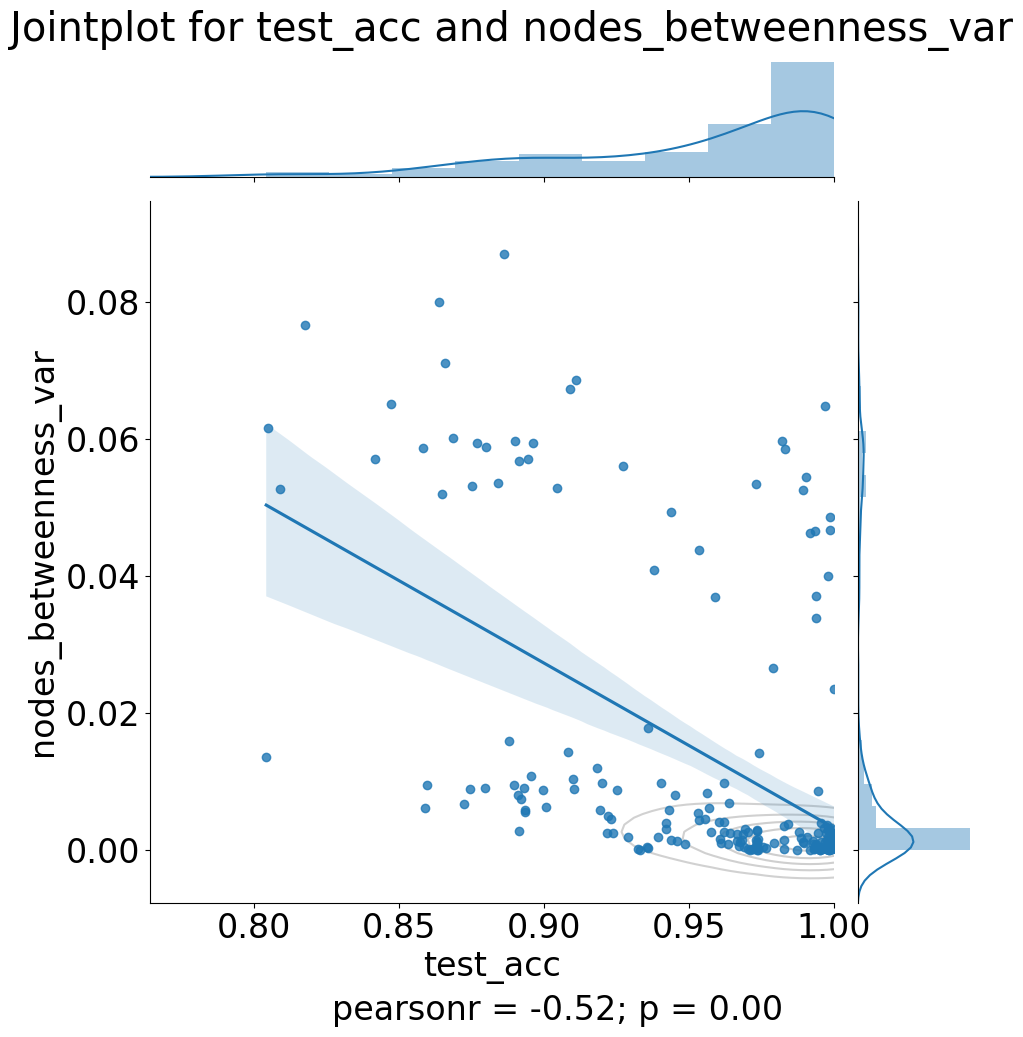
\includegraphics[width=\linewidth]{images/results/random/gru/jointplot_test_acc_nodes_betweenness_var.png}
        \caption{Correlation between test\_acc and node betweenness in base random graph} \label{fig:jp_gru_node_bn}
    \end{subfigure}

\caption[Correlation between test accuracy of GRU and its different graph and recurrent network properties - 2]{Correlation between test accuracy of GRU and its different graph and recurrent network properties - 2} \label{fig:gru_correlation_2}
\end{figure}
